
\section{\large Making more of less}

\subsection{Ex. 12.6 in the book - again}
%For each problem, outline the problem in your own words, your approach, what you did and why you did it.
The task is to design a digital lowpass filter with prewarping that fulfils the following conditions:
\begin{enumerate}
  \item Unit DC gain $G_0 =1$.
  \item Passband angular corner frequency $\omega_p = 10 \, \textnormal{rad/s}$ with passband gain $G_p = 0.785$.
  \item Stopband angular corner frequency $\omega_s = 15 \, \textnormal{rad/s}$ with stopband rejection $G_s = 0.2818$.
  \item Nyquist frequency given by the angular frequency $\omega_h = 35 \, \textnormal{rad/s} =2\pi f_h$.
\end{enumerate}
The condition on the Nyquist frequency implies a sampling frequency of $f_s = \omega_h/\pi \approx 11.14\, [Hz]$. A lowpass Butterworth filter can be designed to fulfil the specifications above by calculating the required filter order $n$ and cut-off frequency $\omega_c$. These two parameters were determined by using the \texttt{buttord} function and the Butterworth filter coefficients were generated using \texttt{butter}. Note that these functions, when used for digital filter design, prewarp all frequencies by default. The magnitude and phase response of the resulting filter is shown in Figure~\ref{fig:ButterFilter}.

%Show the amplitude and phase response of the resulting filter together with the filter specifications in the title of the plot.
\begin{figure}
\center
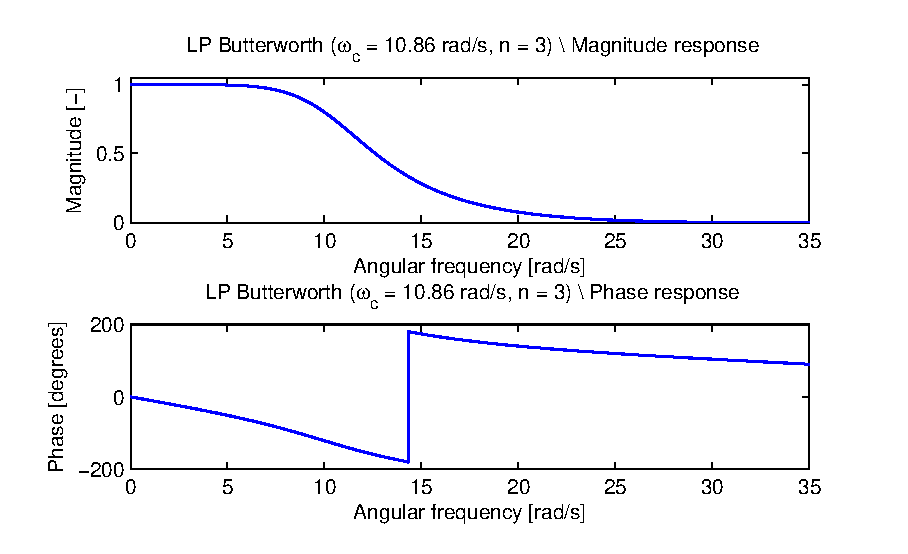
\includegraphics[scale=1]{ButterFilter.eps}
\caption{Magnitude and phase response of the transfer function $H$.}
\label{fig:ButterFilter}
\end{figure}

%Write down the transfer function of the resulting filter and specify the filter type.
\noindent The transfer function $H$ for this filter as determined by MATLAB is approximately
\begin{align*}
H(z) = \frac{b(z)}{a(z)} \approx \frac{0.0538 + 0.1613 z^{-1} + 0.1613 z^{-2} +	0.0538 z^{-3}}{1.0000 - 1.1010z^{-1} +0.6584z^{-2} -0.1273z^{-3}}
\end{align*}
where the cut-off angular frequency is approximately $\omega_c = 10.86 \, \textnormal{rad/s}$, the filter order is $n=3$
and the filter type is (by fulfilling the specifications as required) a lowpass Butterworth filter. A plot of the poles and zeros of $H$ is shown in Figure~\ref{fig:ButterPoleZero}.

\begin{figure}
\center
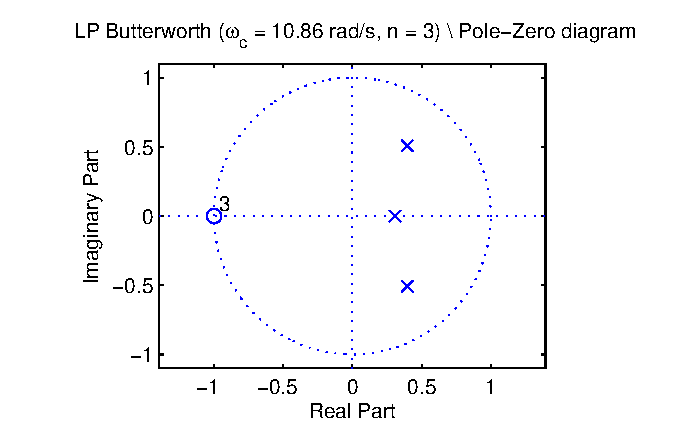
\includegraphics[scale=1]{ButterPoleZero.eps}
\caption{Poles and zeros of the transfer function $H$.}
\label{fig:ButterPoleZero}
\end{figure}

\noindent The manual mathematical derivation proceeds as follows: Let $T = \frac{1}{f_s}$ be the sampling period, then prewarping the angular corner frequencies $\omega_p$ and $\omega_s$ gives
\begin{align*}
\omega_p' &= \frac{2}{T} \tan\Big(\frac{\omega_p T}{2}\Big) \approx 10.7303 \, [s]^{-1} \\
\omega_s' &= \frac{2}{T} \tan\Big(\frac{\omega_s T}{2}\Big) \approx 17.7691 \, [s]^{-1} 
\end{align*}
and using $\omega_p'$ and $\omega_s'$ the approximate filter order can be calculated
\begin{align*}
\left.
\begin{array}{ll}
G_p = \big(1+(\frac{\omega_p'}{\omega_c'})^{2n}\big)^{-1/2} \\
G_s = \big(1+(\frac{\omega_s'}{\omega_c'})^{2n}\big)^{-1/2}
\end{array}
\right\} 
\quad
\Rightarrow
\quad
n = \frac{1}{2}\frac{\ln\big(\frac{G^{-2}_p-1}{G^{-2}_s-1}\big)}{\ln\big(\frac{\omega_p'}{\omega_s'}\big)}
\approx
2.89
\end{align*}
Therefore $n=3$ is chosen and the filter order gives the warped cut-off frequency
\begin{align*}
\omega_c' = \omega_s' (G_s^{-2}-1)^{-\frac{1}{2n}} \approx 11.8114 \, [s]^{-1} && \omega_c = \frac{2}{T} \arctan \Big(\frac{\omega_c' T}{2}\Big) \approx 10.86 \, [s]^{-1} 
\end{align*}
The resulting analogue transfer function $H_a$ has its three poles at the order $2n$ roots of unity in the left half-plane, that is
\begin{align*}
H_a(s) = \frac{1}{(\frac{s}{\omega_c'}-e^{\frac{4\pi}{6}i})(\frac{s}{\omega_c'}-e^{\frac{6\pi}{6}i})(\frac{s}{\omega_c'}-e^{\frac{8\pi}{6}i})}
\end{align*}
using the bilinear transformation $s = \frac{2}{T} \frac{z-1}{z+1} $, the digital transfer function becomes
\begin{align*}
H(z) = H_a\Big( \frac{2}{T} \frac{z-1}{z+1} \Big) &= \frac{(\omega_c')^3}{(\frac{2}{T} \frac{z-1}{z+1} - \omega_c' e^{\frac{4\pi}{6}i})(\frac{2}{T} \frac{z-1}{z+1} - \omega_c' e^{\frac{6\pi}{6}i})(\frac{2}{T} \frac{z-1}{z+1} - \omega_c' e^{\frac{8\pi}{6}i})} \\
&\approx \frac{0.0538 + 0.1613 z^{-1} + 0.1613 z^{-2} +	0.0538 z^{-3}}{1.0000 - 1.1010z^{-1} +0.6584z^{-2} -0.1273z^{-3}}
\end{align*}
This is as expected. Note that $\omega_c$ agrees with the unwarped cut-off determined by MATLAB.
Note also that the bilinear transformation maps $-1$ into $\infty$ where $H_a$ has a zero of order 3. This explains why $H$ has a zero of order $3$ at $-1$ as Figure~\ref{fig:ButterPoleZero} shows.


\newpage
\subsection{The issue of phase shifts and order}
%Use the filter designed above to process a sinusoidal signal such that the resulting phase shift is zero.
Assuming that a signal must be processed (and also that it is not to be processed in real time) using only the filter designed in the previous step, in a way such that no phase shift is incurred, then one solution is to filter the signal, time-reverse the output, filter and time-reverse again. This results in zero phase shift, but a twice applied magnitude response. \\

\noindent Let $f$ be a signal of length $N_0$ and $\mathcal{P}$ the parity operator $\mathcal{P}f(k)=f(N_0-k-1)$, then
\begin{align*}
\mathcal{F}\mathcal{P}f(n) 
&= \sum^{N_0-1}_{k=0} f(N_0-k-1) e^{-2\pi i\frac{kn}{N_0}} \\
&= \sum^{N_0-1}_{k=0} f(k) e^{-2\pi i \frac{(N_0-k-1)n}{N_0}} = e^{2\pi i \frac{n}{N_0}} \overline{\mathcal{F}f(n)}
\end{align*}
Let $x$ be a signal of length $N_0$ and $X=\mathcal{F}x$, then the filtered signal is $Y(n) = H(e^{2\pi i \frac{n}{N_0}})X(n)$. Time-reversing, filtering and time-reversing again gives the output
\begin{align*}
Z(n) &= e^{2\pi i \frac{n}{N_0}}\overline{H(e^{2\pi i \frac{n}{N_0}})e^{2\pi i \frac{n}{N_0}}\overline{Y(n)}} \\
 &= \overline{H(e^{2\pi i \frac{n}{N_0}})\overline{H(e^{2\pi i \frac{n}{N_0}})X(n)}} \\ 
 &= |H(e^{2\pi i \frac{n}{N_0}})|^2 X(n)
\end{align*}
This shows that the phase is unchanged and also that the magnitude response is applied twice.\\

\noindent The process described above can be executed directly in MATLAB using the \texttt{filtfilt} function. A pure tone was filtered in this way and the result is shown in Figure~\ref{fig:ButterFiltFilt}.

%Plot the original and the processed signals on top of each other.
\begin{figure}[H]
\center
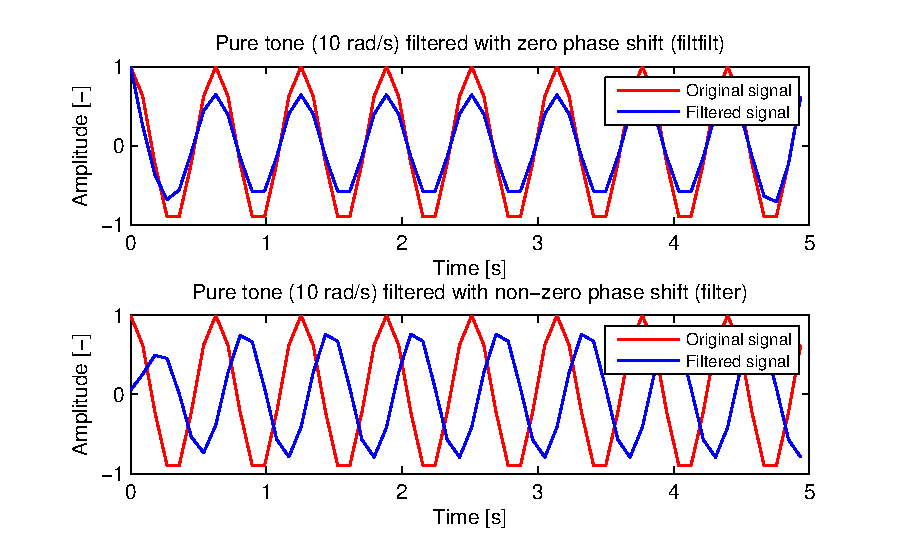
\includegraphics[scale=1]{ButterFiltFilt.eps}
\caption{Filtering a pure tone with zero and non-zero phase shift.}
\label{fig:ButterFiltFilt}
\end{figure}

%What could you do in order to have a filter with approximately twice or three times the order?
\noindent Assuming now that a signal must be processed in such a way that the required filter order is about twice or three times that of the filter designed, while phase shifting is of no importance, then a simple solution is to connect two or three copies of the filter in series (filter cascade). This doubles or triples the filter order, since the resulting transfer function is $H(z)^2$ or $H(z)^3$. Plots of magnitude and phase responses of cascades of $H$ are given in Figure~\ref{fig:ButterCascade}.

%Plot the corresponding frequency transfer functions on top of each other.
\begin{figure}[H]
\center
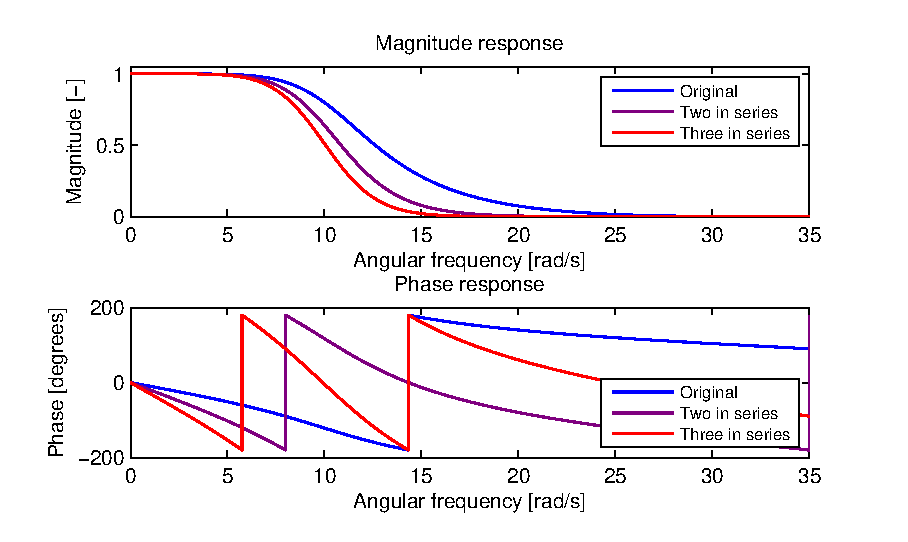
\includegraphics[scale=1]{ButterCascade.eps}
\caption{Magnitude and phase response of cascades of $H$.}
\label{fig:ButterCascade}
\end{figure}


